% https://wiki.physik.uzh.ch/cms/latex:tikz:solenoid
% Author: Izaak Neutelings (June 2018)
\documentclass[border=3pt,tikz]{standalone}

\usepackage{tikz}
\tikzset{>=latex} % for LaTeX arrow head
\usetikzlibrary{calc} 
\usetikzlibrary{patterns,snakes}

\begin{document}
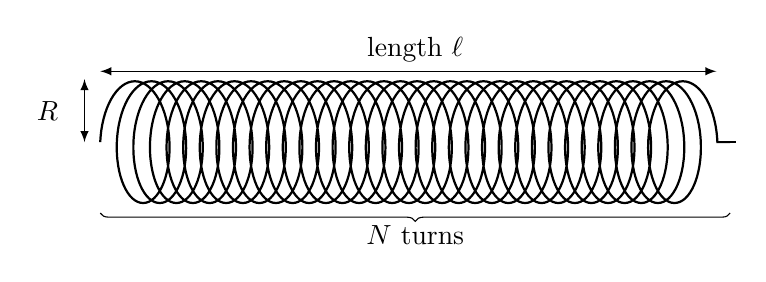
\begin{tikzpicture}[scale=1]
  \def\R{0.8}
  \def\A{11}   % amplitude
  \def\s{6}    % coil segment length
  \def\L{8}    % coil length
  \def\a{0.5}  % coil segment aspect
  \def\dy{0.9} % vertical shift
  \def\dx{0.2} % horizontal shift
  \draw[snake=coil,thick,segment amplitude=2*\A,segment length=\s,segment aspect=\a]
    (0,0) -- (\L,0);
  \draw[<->,shorten >=5]
    (0,\dy) -- (\L,\dy) node[midway,above] {length $\ell$};
  \draw[snake=brace,mirror snake,segment amplitude=3]
    (0,-\dy) -- (\L,-\dy) node[midway,below=1] {$N$ turns};
  \draw[-,thick]
    (\L,0) -- (1.01*\L,0); % coil extension
  \draw[<->]
    (-\dx,0) -- (-\dx,\R) node[midway,left=6] {$R$};
\end{tikzpicture}
\end{document}